\section{Idiotenseite}
\subsection{Einheitskreis}
\begin{center}
	\includegraphics[width=0.6\columnwidth]{Images/einheitskreis}\\
	Punkte auf Kreis [$\cos(\alpha), \sin(\alpha), \tan(\alpha)$]
\end{center}

\noindent\textbf{Grad zu Bogen}:
\[
rad = grad \cdot \frac{\pi}{180}
\]
\noindent\textbf{Bogen zu Grad}:
\[
grad = rad \cdot \frac{180}{\pi}
\]

\subsection{Ableitungen}
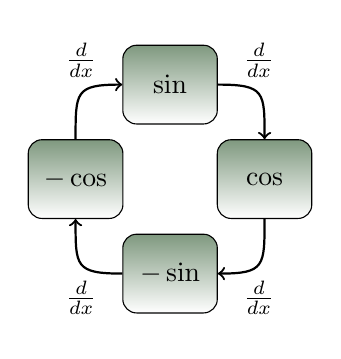
\begin{tikzpicture}
	[	inner sep = 2mm,
	sin/.style={rectangle,minimum width=1.2cm,minimum height=1cm,rounded corners=5pt,draw=black,top color=green!20!black!50},
	abl/.style={rectangle}
	]
	\node at (1.2,0) (sin1) [sin] {$\sin$};
	\node at (0,-1.2) (cos2) [sin] {$-\cos$};
	\node at (1.2,-2.4) (sin2) [sin] {$-\sin$};
	\node at (2.4,-1.2) (cos1) [sin] {$\cos$};
	
	\draw[thick,black,->] (sin1.east) .. controls +(right:0.6cm) and +(up:0.6cm) ..  (cos1.north)
	node [pos=0.5,above](abl) {$\frac{d}{dx}$};
	\draw[thick,black,->] (cos1.south) .. controls +(down:0.6cm) and +(right:0.6cm) .. (sin2.east)
	node [pos=0.5,below](abl) {$\frac{d}{dx}$};
	\draw[thick,black,->] (sin2.west) .. controls +(left:0.6cm) and +(down:0.6cm) .. (cos2.south)
	node [pos=0.5,below](abl) {$\frac{d}{dx}$};
	\draw[thick,black,->] (cos2.north) .. controls +(up:0.6cm) and +(left:0.6cm) .. (sin1.west)
	node [pos=0.5,above](abl) {$\frac{d}{dx}$};
\end{tikzpicture}

\subsection{Doppel- und Halbwinkel}	
$\sin(2a)=2\sin(a)\cos(a)$\\
$\cos(2a)=\cos^2(a)-\sin^2(a)=2\cos^2(a)-1=1-2\sin^2(a)$\\
$\cos^2 \left(\frac{a}{2}\right)=\frac{1+\cos(a)}{2} \qquad
\sin^2 \left(\dfrac{a}{2}\right)=\frac{1-\cos(a)}{2}$

\subsection{Periodizität}
$\cos(a+k\cdot2\pi)=\cos(a) \qquad \sin(a+k\cdot2\pi)=\sin(a) \qquad
(k \in \mathbb{Z})$

\subsection{Additionstheoreme}
$\sin(a \pm b)=\sin(a) \cdot \cos(b) \pm \cos(a) \cdot \sin(b)$\\
$\cos(a \pm b)=\cos(a) \cdot \cos(b) \mp \sin(a) \cdot \sin(b)$\\	
$\tan(a \pm b)=\dfrac{\tan(a) \pm \tan(b)}{1 \mp \tan(a) \cdot \tan(b)}$\\
$\sin(a)\sin(b)=\frac{1}{2}(\cos(a-b)-\cos(a+b))$\\
$\cos(a)\cos(b)=\frac{1}{2}(\cos(a-b)+\cos(a+b))$\\
$\sin(a)\cos(b)=\frac{1}{2}(\sin(a-b)+\sin(a+b))$\\

\newpage

\begin{landscape}
	\section{Eigenschaften Funktionen}
	\begin{center}
		\includegraphics[width=\linewidth]{./Images/eigenschaften.png}
	\end{center}
\end{landscape}

